\section{Introduction}

Second generation neural networks achieve impressive results
on all tasks that can collectively be identified as data classification.
As of the time of writing, second generation convolutional networks
continue dominating every ImageNet classification challenge of the last
years~\cite{ILSVRC15}.

\subsection{Limits of current approaches to AI}
There are still types of tasks that no deep learning topology or
technique has been able to tackle so far. Adversarial evaluations of reading comprehension
systems indicate that neural networks that excell at evaluating carefully
prepared data prove to be extremely fragile when encountering organic ``noise''
information~\cite{DBLP:journals/corr/JiaL17}.
The practice of splitting learning into separate training and application steps
means that a traditional neural network is unable to continuously learn while working.
This way, new information cannot be aquired dynamically as it has to be spoon-fed in the
form of carefully prepared test data.
Further limitations of current deep learning strategies have been compiled by 
Gary Marcus~\cite{DBLP:journals/corr/abs-1801-00631}.

One way to interpret these limitations is as an expression of the growing discrepancy between
biological neural networks and the mentioned systems~\cite{Paugam-Moisy2012}.

\subsection{General Intelligence in nature}
In light of these dissatisfactions with the current state of AI, we take a deliberate step back 
from current research and ask ourselves what the goal of artificial intelligence research should actually be.
In our opinion, AI is not about the automation of simple tasks or the labeling of pictures. 
Artificial Intelligence should be about intelligence. And the only form of intelligence that can truly
stimulate and satisfy the human being is one, that is similar to its own inner workings: A General Intelligence (GI),
flexible enough to adapt to an everchanging environment, enduring enough to continuously learn and change its approach.
So far, the only general intelligence that we know of resides within our own heads. It is therefore tempting to
build an Artificial General Intelligence (AGI) by simply replicating the human brain in an artificial setting. In practice
however, this bottom-up approach proves to be only advantageous when studying in situ micromodels and 
their effects in isolation~\cite{Dudai2014}. 

\subsection{The scale of abstraction}
One can imagine all approaches to intelligence as if on a scale of abstraction.
One end of this scale, the extreme denominating the absolute lack of any abstraction, is the human brain.
The other end has no clear extreme as there cannot be a maximum of abstraction~(To do: Cite philosopher) and must 
be defined arbitrarily. We choose the well-known example of the first-generation perceptron for this task as its
shortcomings have been described in great detail by various sources~\cite{Anderson1995}.
Our challenge as seekers of General Intelligence is now to analyze various approaches and approximate their position on
the scale on order to deduce the abstraction level that will lead to a simulation capable of AGI\@.

We interpret the limitations of bottom-up brain simulations as a concequence of choosing the wrong level of abstraction, 
namely one that is too low. In contrast, if we want to place the second-generation approach of Artificial Neural Networks as we train today on
the same spectrum of abstraction, they must naturally be placed on the opposite side, as indicated by their reductionist
principles. The second-generation systems are too abstract. The optimal level of abstraction necessary for AGI must 
therefore lie between these two extremes. The solution is neither a chemical copy of the brain, nor does it abstract 
away the absolute statefulness of the brain as a function of internal state, sensory inputs and time.
Third-generation spiking neural networks present themselves as a good compromise between
realism and flexibility for conceptual modeling~\cite{Paugam-Moisy2012}. However, just choosing the appropiate
neural model is not enough. 

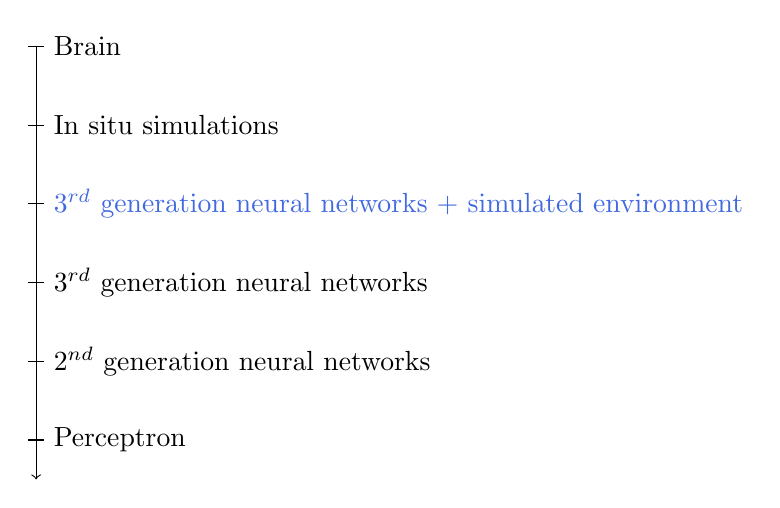
\begin{tikzpicture}
    \draw[<-] (0, -0.5) -- (0, 5);
    \draw (-0.1, 5) -- (0.1, 5) node[right] {Brain};
    \draw (-0.1, 4) -- (0.1, 4) node[right] {In situ simulations};
    \draw (-0.1, 3) -- (0.1, 3) node[right] {\color{RoyalBlue}$3^{rd}$ generation neural networks + simulated environment};
    \draw (-0.1, 2) -- (0.1, 2) node[right] {$3^{rd}$ generation neural networks};
    \draw (-0.1, 1) -- (0.1, 1) node[right] {$2^{nd}$ generation neural networks};
    \draw (-0.1, 0) -- (0.1, 0) node[right] {Perceptron};
\end{tikzpicture}
